\documentclass[xcolor=svgnames]{beamer}
\usetheme{Madrid}
%\useoutertheme{miniframes} % Alternatively: miniframes, infolines, split
\useinnertheme{circles}

\usepackage{mathpazo}

\usepackage{xurl}

%Define the colurs
\definecolor{Champagne}{RGB}{253, 235, 191}
\definecolor{RoseQuartz}{RGB}{243, 184, 183}
\definecolor{BlueGray}{RGB}{85, 104, 144}
\definecolor{Black}{RGB}{31, 32, 32}

\definecolor{PrussianBlue}{RGB}{0, 51, 102}
\definecolor{LincolnGreen}{RGB}{25, 89, 5}
\definecolor{SapphireSplendour}{RGB}{36, 37, 185}

\renewcommand{\emph}[1]{\textcolor{DarkMagenta}{\textbf{#1}}}
\newcommand{\presenter}[1]{\textcolor{SapphireSplendour}{\textbf{#1}}}

%Instead of using \usecolortheme define yours
\setbeamercolor{structure}{fg=DarkBlue}
\setbeamercolor{palette primary}{bg=LightSteelBlue,fg=Black}
\setbeamercolor{palette secondary}{bg=Plum,fg=Black}
\setbeamercolor{palette tertiary}{bg=RoseQuartz,fg=Black}

%Title page things
\setbeamercolor{title}{bg=RoseQuartz,fg=Black}
\setbeamerfont{title}{series=\bfseries}
\title[Degree-Constrained Social Network Design]{Design and Optimization of Degree-Constrained Social Networks}
\author[C.~Brett and \presenter{L.~M.~B.~Varona}]{
  \emph{Luis M.~B.~Varona}\inst{a,b,c} \\
  {\footnotesize Joint work with Craig Brett\inst{a}}
}
\institute[MtA]{
  2026 Science Atlantic Math., Stats., \& CS Conference \\
  University of New Brunswick SJ, Saint John, NB
}
\date[24 October 2026]{24 October 2026}
\titlegraphic{\vspace*{-0.4cm}
\includegraphics[width=4cm]{assets/mta-logo.png}}
\setbeamertemplate{navigation symbols}{} %For clearing the symbols at the bottom

%Itemize color and shape change
\setbeamertemplate{itemize item}[circle]
\setbeamertemplate{itemize subitem}[circle]
\setbeamercolor{itemize item}{fg=LincolnGreen}
\setbeamercolor{itemize subitem}{fg=SapphireSplendour}

%Enumerate color change
\setbeamercolor{item projected}{fg=white,bg=BlueGray}

%Frame Title Change
\setbeamercolor{frametitle}{fg=Black,bg=RoseQuartz}
\setbeamerfont{frametitle}{series=\mdseries,parent=structure}

%Theorems and blocks
\setbeamercolor{block title}{use=structure,fg=Black,bg=LightSteelBlue}
\setbeamercolor{block body}{use=structure,fg=black,bg=WhiteSmoke}
\addtobeamertemplate{block begin}{%
		\setlength{\textwidth}{0.9\textwidth}%
}{}

\usepackage[safe]{tipa}

\usepackage{ragged2e} %For justifying the text
\justifying

\usepackage[skins,theorems]{tcolorbox} %colored boxes for equations
\tcbset{highlight math style={enhanced,colframe=Black,colback=Champagne,arc=0pt,boxrule=1pt}}

\usepackage{amssymb} %Symbols from the American Mathemetical Society
\usepackage{amsmath} %Equations
\usepackage{mathtools} %Extention to amsmath
\usepackage{mathrsfs} %For curly L in Cartan's equation
\usepackage{dsfont}
\usepackage{physics} %For abs

\usepackage{caption} %for captions

\setbeamerfont{footnote}{size=\scriptsize}

% nice-looking footnotes in slides
\usepackage[absolute,overlay]{textpos}
\newenvironment{reference}[2]{%
  \begin{textblock*}{\textwidth}(#1,#2)
  \footnotesize\it\bgroup\color{DarkBlue}}{\egroup
\end{textblock*}}

% shrinks its argument only if it is wider than the line
\newcommand{\fitwidth}[1]{\resizebox{\ifdim\width>\linewidth\linewidth\else\width\fi}{!}{#1}}

\def\I{\mathbb{1}}
\def\O{\mathbb{O}}
\def\C{\mathbb{C}}
\def\N{\mathbb{N}}
\def\Z{\mathbb{Z}}
\def\Q{\mathbb{Q}}
\def\R{\mathbb{R}}
\def\E{\mathbb{E}}
\def\F{\mathbb{F}}

\def\B{\mathcal{B}}
\def\D{\mathcal{D}}
\def\Ein{\mathcal{E}}
\def\K{\mathcal{K}}
\def\Lin{\mathcal{L}}
\def\M{\mathcal{M}}
\def\Sin{\mathcal{S}}
\def\U{\mathcal{U}}
\def\V{\mathcal{V}}
\def\W{\mathcal{W}}
\def\X{\mathcal{X}}
\def\Y{\mathcal{Y}}

\def\a{\mathbf{a}}
\def\b{\mathbf{b}}
\def\cc{\mathbf{c}} % To avoid overriding diacritics
\def\d{\mathbf{d}}
\def\e{\mathbf{e}}
\def\p{\mathbf{p}}
\def\q{\mathbf{q}}
\def\rr{\mathbf{r}} % To avoid overriding diacritics
\def\uu{\mathbf{u}} % To avoid overriding diacritics
\def\vv{\mathbf{v}} % To avoid overriding diacritics
\def\w{\mathbf{w}}
\def\x{\mathbf{x}}
\def\y{\mathbf{y}}
\def\z{\mathbf{z}}
\def\0{\mathbf{0}}
\def\1{\mathbf{1}}

\makeatletter
\renewcommand{\enumerate}{%
  \ifnum\@enumdepth>3\relax\@toodeep\else
    \advance\@enumdepth\@ne
    \edef\@enumctr{enum\romannumeral\the\@enumdepth}%
    \advance\@itemdepth\@ne
  \fi
  \beamer@computepref\@enumdepth
  \edef\beamer@enumtempl{enumerate \beameritemnestingprefix item}%
  \@ifnextchar[{\beamer@@enum@}{\beamer@enum@}}
\renewcommand{\beamer@computepref}[1]{%
  \let\beameritemnestingprefix\@empty
  \ifcase#1\or\or\def\beameritemnestingprefix{sub}\or\def\beameritemnestingprefix{subsub}\or\def\beameritemnestingprefix{subsub}\else\@toodeep\fi}
\setlength{\leftmarginiv}{\leftmarginiii}
\def\@listiv{\@listiii\leftmargin\leftmarginiv}
\renewcommand{\insertsubenumlabel}{\alph{enumii}}
\renewcommand{\insertsubsubenumlabel}{\ifnum\@enumdepth>3 \Alph{enumiv}\else\roman{enumiii}\fi}
\makeatother

\begin{document}

\section{Opening Remarks}

{
    \setbeamertemplate{footline}{} %deleting the slide number from the title page
    \begin{frame}
        \vspace*{-0.8cm}
        \titlepage
        \begin{reference}{10mm}{83mm}
            \rule{4cm}{0.5pt} \\
            \scriptsize
            \textsuperscript{a}Department of Economics, Mount Allison University\\
            \textsuperscript{b}Department of Politics \& International Relations, Mount Allison University\\
            \textsuperscript{c}Department of Mathematics \& Computer Science, Mount Allison University\par
        \end{reference}
    \end{frame}
}
\addtocounter{framenumber}{-1}	%resetting the counting for the slides

{
    \setbeamercolor{background canvas}{bg=PrussianBlue}
    \setbeamercolor{normal text}{fg=white}
    \setbeamercolor{itemize item}{fg=Khaki}
    \usebeamercolor[fg]{normal text}

    \begin{frame}
        \frametitle{Land Acknowledgement}
        \begin{itemize}
            \item The land on which we gather is the traditional unceded territory of the W\textschwa last\textschwa kwiyik (Maliseet), covered by the ``Treaties of Peace and Friendship'' which W\textschwa last\textschwa kwiyik (Maliseet), Mi'kmaq and Passamaquoddy Peoples first signed with the British Crown in 1726\vfill
            \item The treaties did not deal with surrender of lands and resources but in fact recognized Mi'kmaq and W\textschwa last\textschwa kwiyik (Maliseet) title and established the rules for what was to be an ongoing relationship between nations\vfill
            \item Furthermore, much of this research was conducted in Sackville, NB (the unceded ancestral lands of the Mi'kmaw people) and Montreal, QC (the traditional territory of the Kanien'keh\`a:ka)
        \end{itemize}
    \end{frame}
}

\section{Background}

\begin{frame}{What Are Socioeconomic Networks?}
    \begin{itemize}
        \item \emph{Socioeconomic networks} are \emph{graphs} in which nodes represent agents/infrastructure/etc. and edges represent ties/links\vspace*{0.1cm}
        \item Networks are ubiquitous in society and the economy: social media, transportation systems, electrical grids, supply chains\vspace*{0.1cm}
        \item Designing and optimizing networks for \emph{efficiency} and \emph{connectivity} is a focus in computational and algorithmic economics
    \end{itemize}
    \vspace*{-0.1cm}
    \begin{figure}
        \centering
        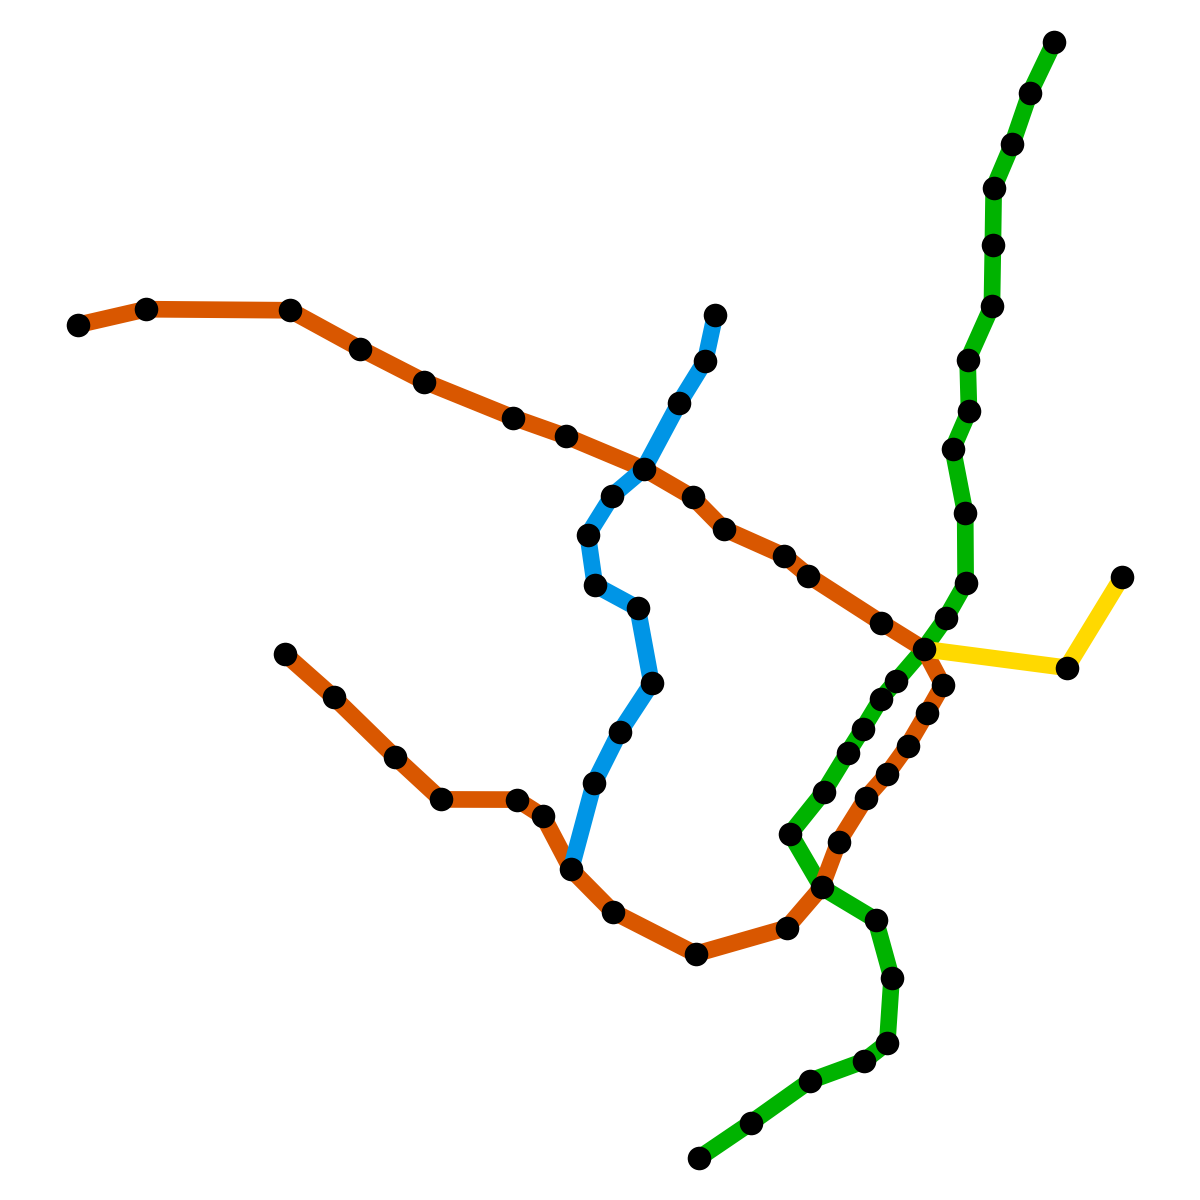
\includegraphics[height=4.1cm]{assets/montreal_metro.png}
        \vspace*{-0.05cm}
        \caption{The \emph{Montreal Metro} represented as a network/graph, drawn to scale.}
    \end{figure}
    \vspace*{-0.3cm}
\end{frame}

\begin{frame}{What Are Communication Networks?}
    \begin{itemize}
        \item Consider a specific type of network. Fix $n \ge 3$ and $X \in (0, 1)$, then:\vspace*{0.15cm}
        \begin{itemize}
            \item A (max-strength) \emph{communication network} is a graph $G$ with $n$ agents in which each agent forms one weight-$X$ edge to another\vspace*{0.15cm}
            \item Although edge formation is directed, ``value'' flows both ways between agents and \emph{decays exponentially} with distance\vspace*{0.15cm}
            \item Assume no co-sponsorship of edges, so each connected component is \emph{unicyclic}: a cycle with pendant trees attached to it\vspace*{0.15cm}
        \end{itemize}
        \item \emph{Payoff} of agent $u$ (``how close'' it is to all other agents):
        \begin{align*}
            \varphi_G(u) \coloneqq \sum_{v \in V(G) \setminus \{u\}} X^{d_G(u,v)}
        \end{align*}\vfill
        \item \emph{Value} of network $G$ (for chemists, twice its Hosoya polynomial at $X$):
        \begin{align*}
            \V(G) \coloneqq \sum_{u \in V(G)} \varphi_G(u) = 2 \sum_{\{u, v\} \subseteq V(G),\, u \ne v} X^{d_G(u,v)} = 2 H(G, X)
        \end{align*}
    \end{itemize}
\end{frame}

\begin{frame}{Degree-Unconstrained Networks}
    \begin{itemize}
        \item \emph{Efficient:} Network maximizes $\V(G)$ given fixed \emph{constraints} $n$ and $X$\vspace*{0.25cm}
        \item \emph{Nash:} Every agent maximizes payoff given all other agents' strategies\vspace*{0.25cm}
        \item Traditionally, node degree (both incoming and outgoing) is unconstrained; efficient networks thus have very \emph{low diameter}
    \end{itemize}
    \vspace*{0.1cm}
    \begin{figure}
        \centering
        \fbox{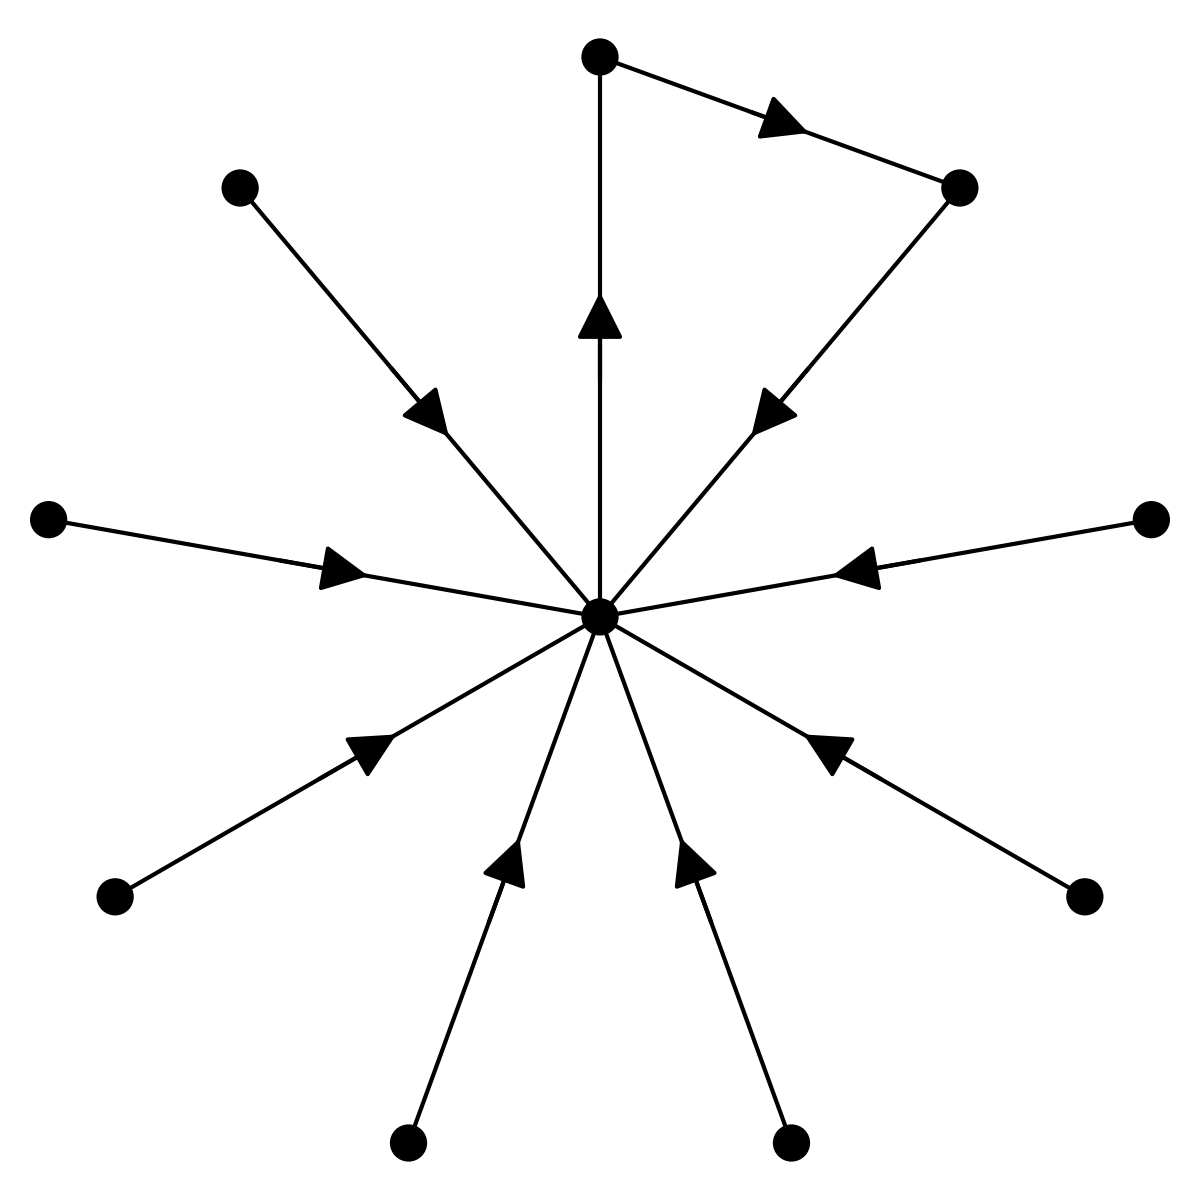
\includegraphics[height=3.8cm]{assets/kakkar_flower_n10.png}}
        \caption{For all $n \ge 6$ and $X \in (0, 1)$: efficient \& connected $\iff$ \emph{star plus edge} [\href{https://doi.org/10.1007/s12626-025-00188-4}{\textcolor{magenta}{Kak25}}]. (We show via partitions that this beats disconnected networks too.)}
    \end{figure}
    \vspace*{-0.3cm}
\end{frame}

\begin{frame}{Imposing Degree Constraints}
    \begin{itemize}
        \item \emph{Real world:} What if a ``central'' agent malfunctions? What if a person/firm/station is not capable of relaying so much data?\vspace*{0.15cm}
        \item Impose a \emph{degree constraint}: a cap $D \in \{2, 3, \ldots, n - 2\}$\vspace*{0.15cm}
        \item Now, larger cycles with many small pendant trees are efficient (cf. a star plus an edge: a small cycle with a large height-$1$ tree)
    \end{itemize}
    \vspace*{0.1cm}
    \begin{figure}
        \centering
        \fbox{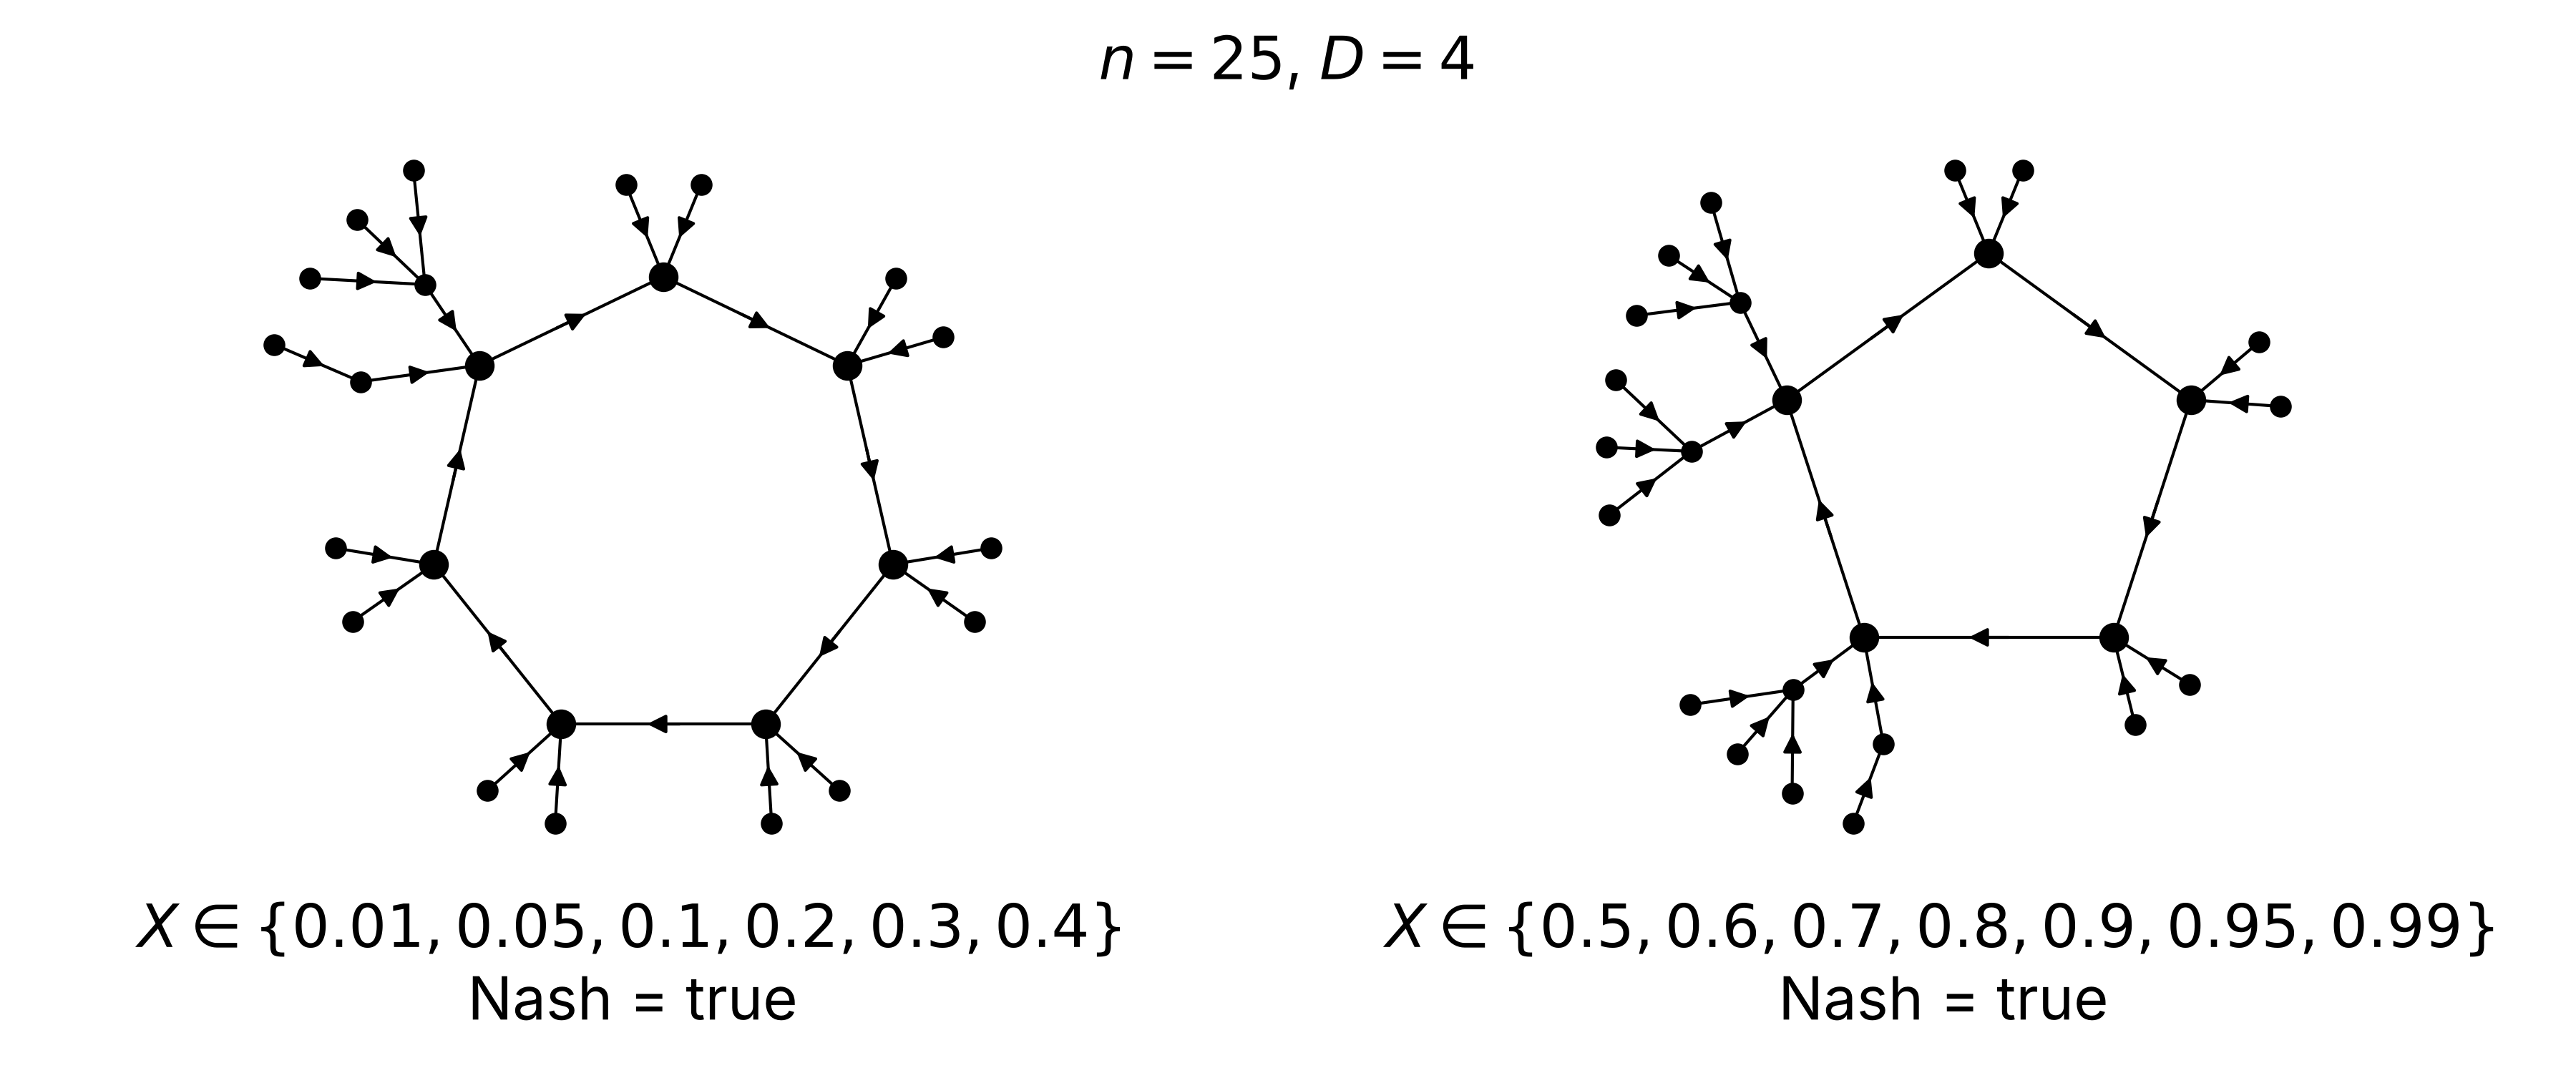
\includegraphics[height=3.9cm]{assets/efficient_D4_n25.png}}
        \caption{The two efficient networks for $n = 25$ and $D = 4$.}
    \end{figure}
    \vspace*{-0.3cm}
\end{frame}

\section{Algorithm Design}

\begin{frame}{Computational Challenges}
    \begin{itemize}
        \item \emph{Many Nash} networks per fixed $(n, D, X)$, so \emph{not} interested in finding all (but can quickly check individual networks in $\Theta(n^3)$ time)\vspace*{0.15cm}
        \item Only a \emph{few efficient} ones, which we \emph{do} want, but difficult to find:\vspace*{0.15cm}
        \begin{itemize}
            \item Infinitely many $X \in (0, 1)$ per fixed $(n, D)$ (still have \emph{not solved} this)\vspace*{0.15cm}
            \item The number of unlabelled graphs on $n$ nodes grows superexponentially: $\lvert \mathcal{G}_n \rvert \in \Theta{\left(2^{\binom{n}{2}} / n!\right)}$ (we have \emph{solved} this!)
        \end{itemize}
    \end{itemize}
    \vspace*{0.1cm}
    \begin{figure}
        \centering
        
\includegraphics[height=3.6cm]{assets/naomi_sleepy_rats_comp.jpg}
        \caption{My friend Naomi's rats: \emph{Parsnip} (left), \emph{Arugula} (middle), and \emph{Clove}.}
    \end{figure}
    \vspace*{-0.3cm}
\end{frame}

\begin{frame}{Algorithm Setup (Part 1)}
    Design an $O\bigl(2.9558^n \cdot \sqrt{n}\bigr)$ algorithm to find all efficient connected networks for fixed $(n, D, X)$. (Given all connected solutions up to $n$, can then check every \emph{partition} $n = \sum n_i$ and compare sums $\sum \V_{n_i}^*$ of optimal values.)\vfill
    \begin{itemize}
        \item For $D = 2$: efficient $\iff$ $n$-cycle\vfill
        \begin{itemize}
            \item So, restrict our attention to $n \ge 5$ and $D \ge 3$\vfill
        \end{itemize}
        \item Only three things matter: \emph{cycle size} $m$, shape of \emph{pendant trees} $T_1, T_2, \ldots, T_m$ (including root cycle nodes $c_1, c_2, \ldots, c_m$; trivial trees count), and \emph{positions} of trees on the cycle\vfill
        \begin{itemize}
            \item So, try all possible cycle sizes and all possible ways to make pendant trees from the leftover nodes\vfill
        \end{itemize}
        \item In an efficient connected network, \emph{cycle size is bounded}:
        \begin{align*}
            m \le \beta(n, D) \coloneqq \begin{cases}
                \max\bigl(\lfloor (n + 1) / 2 \rfloor, 5\bigr) & \text{if } D = 3, \\
                \max\bigl(\lfloor n / 2 \rfloor, 5\bigr) & \text{if } D \ge 4.
            \end{cases}
        \end{align*}
    \end{itemize}
\end{frame}

\begin{frame}{Algorithm Setup (Part 2)}
    \begin{itemize}
        \item Decompose a tree's contribution into its \emph{internal value} $\V(T_i)$ and (some coefficient times) its \emph{``value to the cycle''} $\varphi_{T_i}(c_i)$\vfill
        \item Generate \emph{$(D, X, \ell)$-rat trees}: rooted trees $T$ on $\ell + 1$ nodes that\vfill
        \begin{itemize}
            \item follow degree constraints: $(D - 1)$-ary, with $\le D - 2$ nodes in level $1$,\vfill
            \item are not Pareto-dominated in terms of $\V(T)$ and $\varphi_{T}(\text{root})$.\vfill
            \item \emph{Loose} bound on the number of rat trees: $O\bigl(2.9558^{\ell + 1} \cdot (\ell + 1)^{-3/2}\bigr)$\vfill
        \end{itemize}
        \item \emph{Additional pruning:} as we go, branch-and-bound eliminates even more tree choices when building candidate networks\vfill
        \item Placing the trees is a \emph{quadratic assignment problem} (QAP)\vfill
        \begin{itemize}
            \item Finding \emph{all} optimal assignments is \emph{NP-hard}\vfill
            \item But if \emph{sorted} as $\varphi_{T_1}(c_1) \ge \varphi_{T_2}(c_2) \ge \cdots \ge \varphi_{T_m}(c_m)$, then $\cdots{\sim}c_5{\sim}c_3{\sim}c_1{\sim}c_2{\sim}c_4{\sim}\cdots$ (i.e., a \emph{$\pi^*$} assignment) is \emph{a} solution\vfill
            \item So, try to find all efficient connected networks up to cycle size and pendant trees, and just use $\pi^*$\vfill
        \end{itemize}
    \end{itemize}
\end{frame}

\begin{frame}{Example: Pendant Tree QAP}
    \vspace*{-0.1cm}
    \begin{figure}
        \centering
        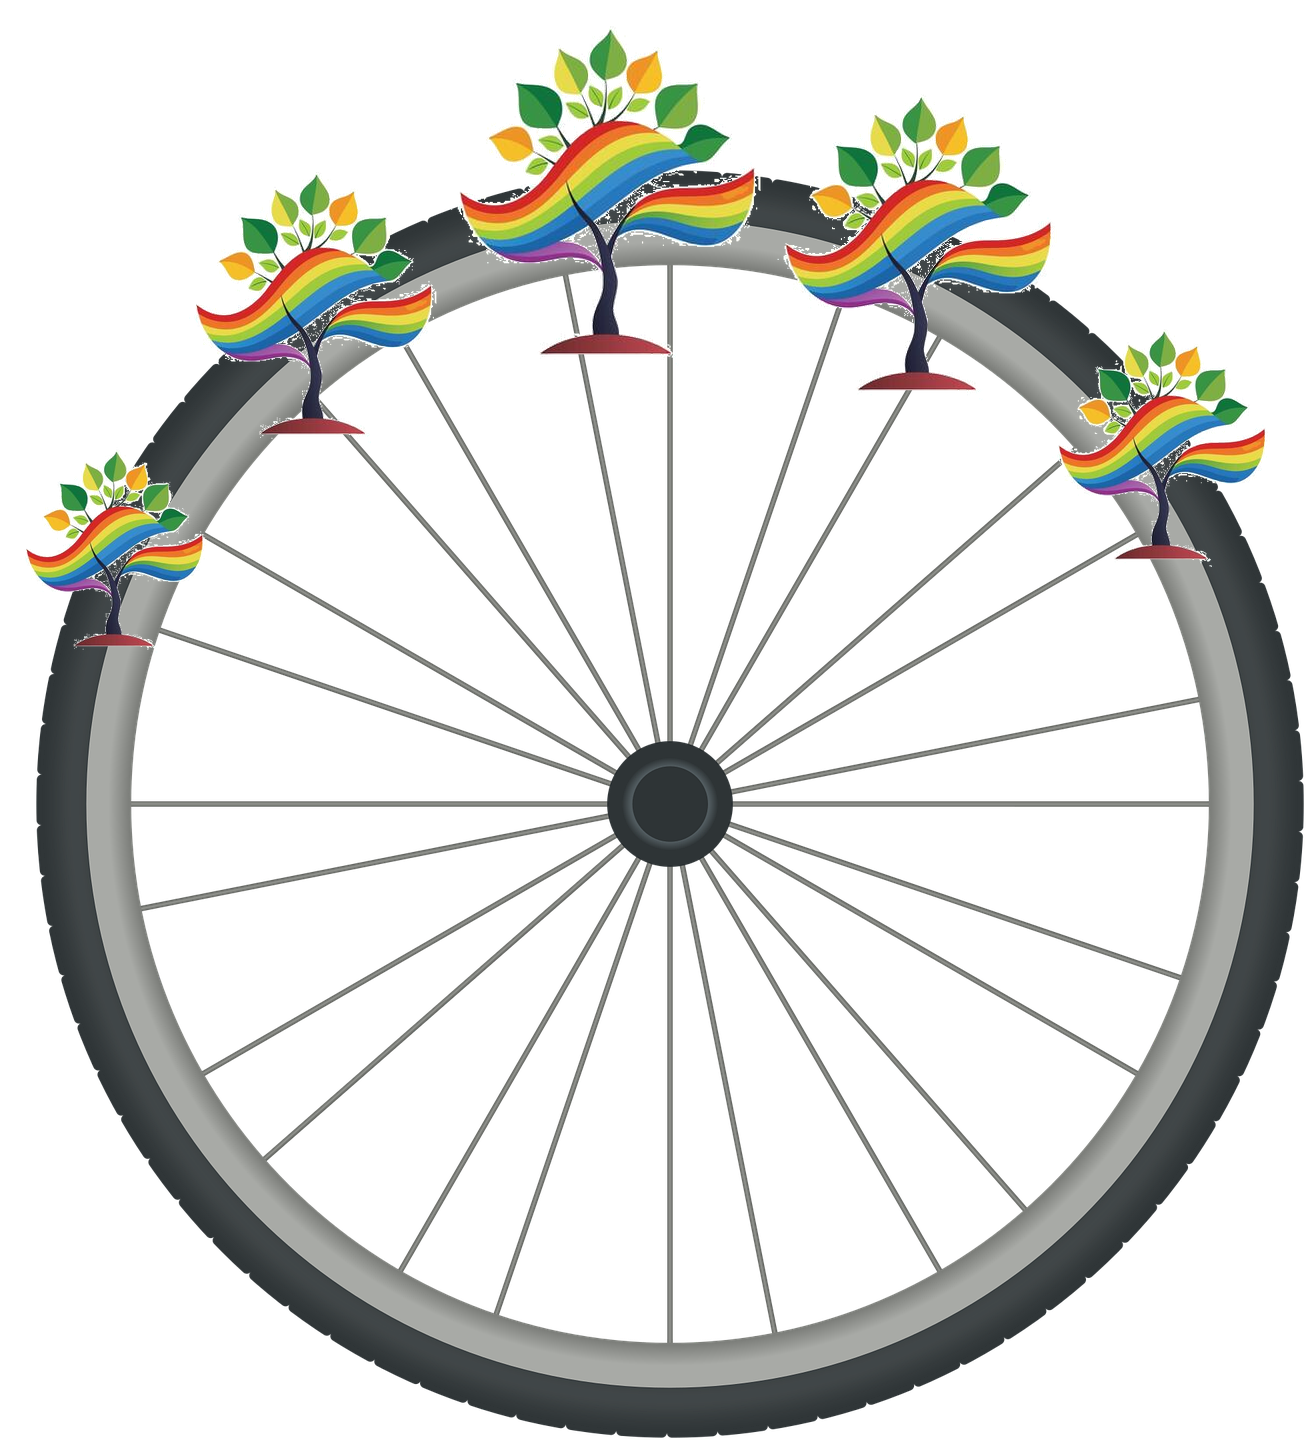
\includegraphics[height=0.78\textheight]{assets/qap_unicycle.png}
        \vspace*{0.1cm}
        \caption{The ``more valuable'' (to the cycle) a tree, the nearer to the middle it is.}
    \end{figure}
\end{frame}

\begin{frame}{Algorithm: Efficient Connected Networks}
    \emph{input:}\quad $n \ge 5$,\quad $D \in \{3, 4, \ldots, n - 2\}$,\quad $X \in (0, 1)$.\vfill
    \begin{enumerate}
        \item set $\Gamma \gets \emptyset$;\quad set $\V^* \gets 0$.\vfill
        \item \emph{for each} $\ell = 0, 1, \ldots, n - 3$ \emph{do}\vfill
        \begin{enumerate}
            \item compute and store $\tau_{\ell} \gets \bigl\{\bigl(T, \V(T), \varphi_T(\text{root})\bigr) \bigm| T \text{ is } (D, X, \ell)\text{-rat}\bigr\}$.
        \end{enumerate}
        \emph{end for}\vfill
        \item \emph{for each} $m = 3, 4, \ldots, \beta(n, D)$ \emph{do}\vfill
        \begin{enumerate}
            \item \emph{for each} partition $(\ell_1, \ell_2, \ldots, \ell_m) \ge \vec{0}$ s.t. $n - m = \sum\ell_i$ \emph{do}\vfill
            \begin{enumerate}
                \item \emph{for each} [unpruned, \underline{unordered} $m$-tuple of data] $\in \tau_{\ell_1} \times \cdots \times \tau_{\ell_m}$ \emph{do}
                \begin{enumerate}
                    \item set $G \gets$ [$m$-cycle with pendant trees $T_1, \ldots, T_m$ under $\pi^*$].
                    \item compute $\mathcal{V} \gets \V(G)$ using stored $\V(T), \varphi_T(\text{root})$ data.
                    \item \emph{if} $\V > \V^*$ \emph{then};\quad set $\Gamma \gets \{(T_1, \ldots, T_m)\}$;\quad set $\V^* \gets \V$.\vfill
                    \emph{else if} $\V = \V^*$ \emph{then};\quad set $\Gamma \gets \Gamma \cup \{(T_1, \ldots, T_m)\}$.\vfill
                    \emph{end if}\vfill
                \end{enumerate}
                \emph{end for}\vfill
            \end{enumerate}
            \emph{end for}\vfill
        \end{enumerate}
        \emph{end for}\vfill
    \end{enumerate}
    \emph{output:}\quad $\Gamma$ (fully describes equivalence classes),\quad $\V^*$ (optimal value).
\end{frame}

\section{Empirical Results}

\begin{frame}{Data and Implications}
    \begin{itemize}
        \item In practice, \emph{significantly faster}: scales as roughly $O(1.3^n)$\vfill
        \item Identified all efficient connected networks for $D \in \{3, 4, 5, 6\}$, $n \le 36$, and $X \in \{0.01, 0.05, 0.1, 0.2, \ldots, 0.8, 0.9, 0.95, 0.99\}$ (\emph{13 values}), as well as up to $n = 43$ for $D = 3$\vfill
        \item Identified interesting Nash networks, both efficient and inefficient (not in scope here, but helpful for our mathematical economics paper)\vfill
        \item Found empirical evidence (not yet proven) for:\vfill
        \begin{itemize}
            \item \emph{Efficient $\implies$ connected} (recursively checked integer partitions of $n$)\vfill
            \item \emph{Complete trees} (i.e., BFS-filled) maximize network value\vfill
            \item \emph{Cycle size} $m$ appears to be \emph{sublinear} in $n$\vfill
            \item Again, a lot of interesting \emph{Nash stuff} not covered here~\ldots
        \end{itemize}
    \end{itemize}
\end{frame}

\begin{frame}{Examples: Efficient Networks}
    \begin{figure}
        \centering
        \fbox{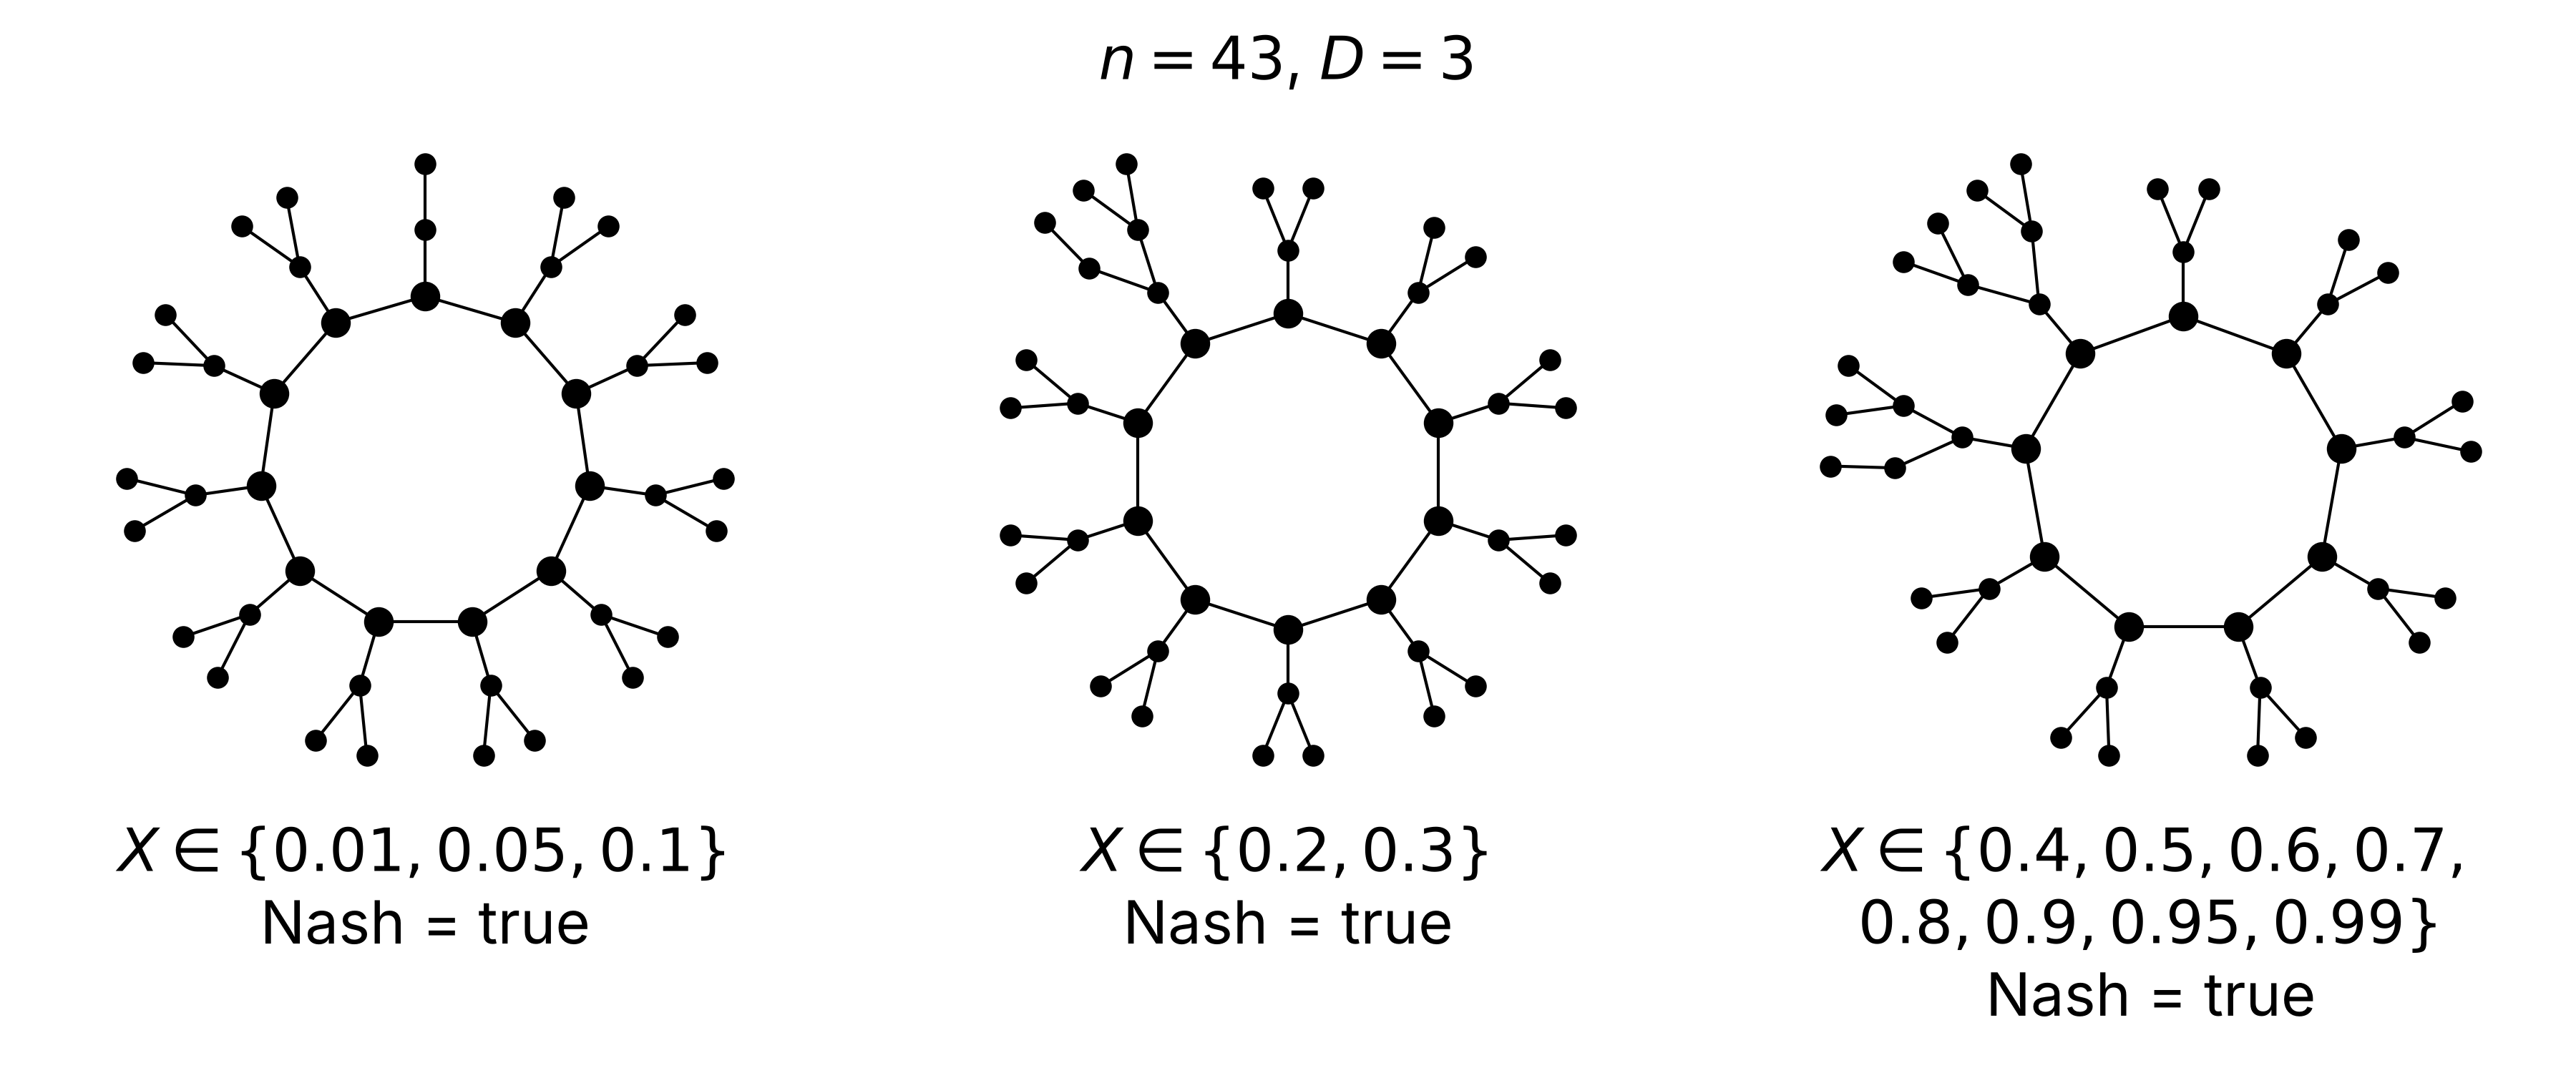
\includegraphics[height=3.35cm]{assets/efficient_D3_n43.png}}

        \vspace*{0.1cm}
        \fbox{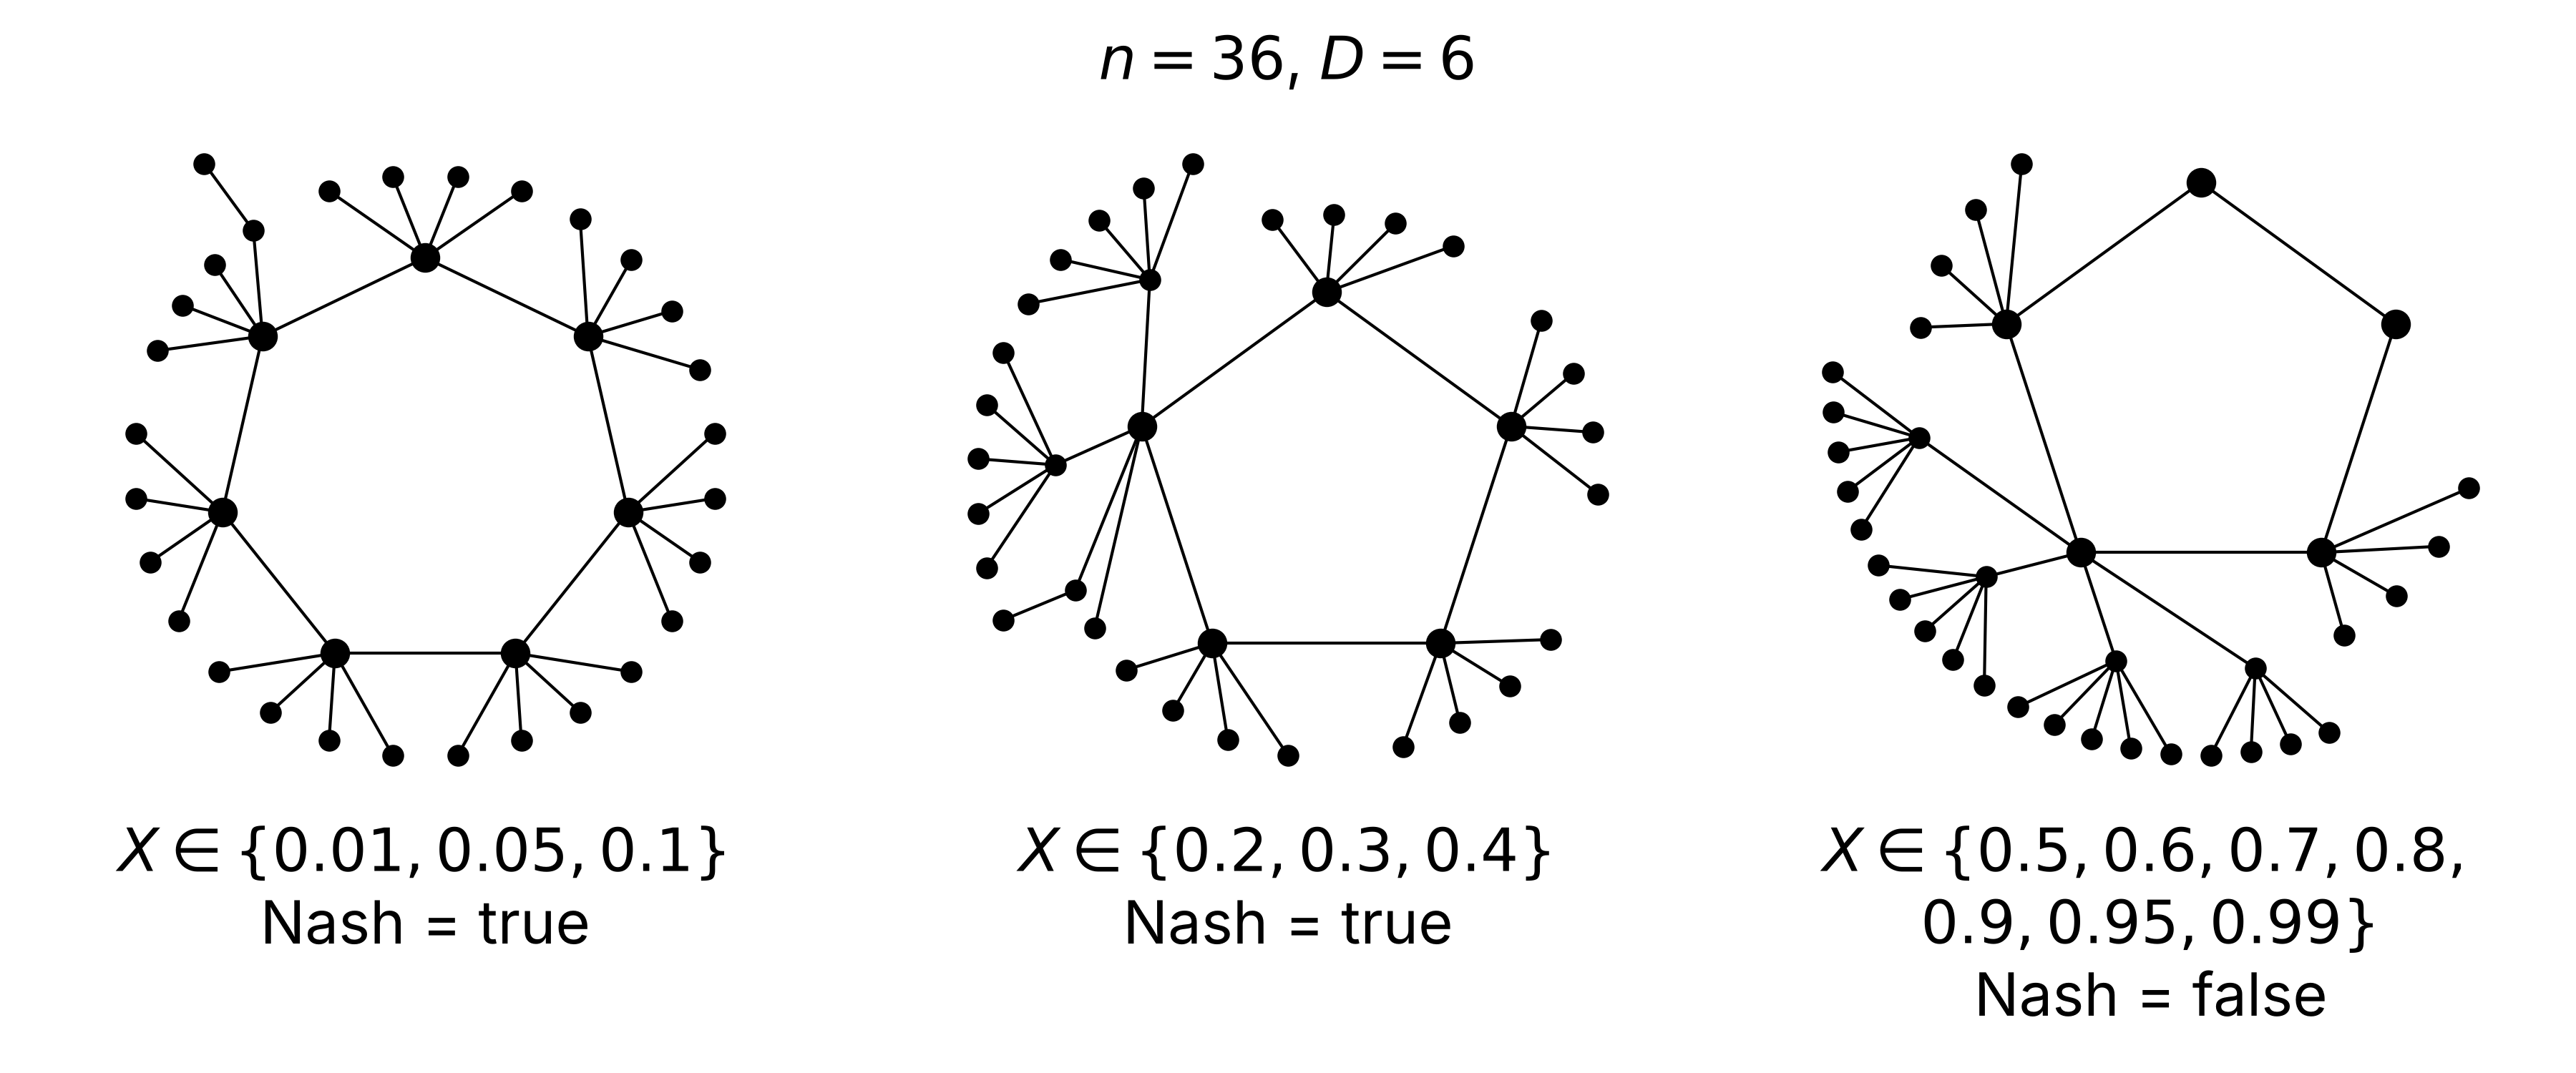
\includegraphics[height=3.35cm]{assets/efficient_D6_n36.png}}

        \vspace*{-0.075cm}
        \caption{Efficient networks exhibiting connectedness and tree completeness.}
    \end{figure}
\end{frame}

\section{Conclusion}

\begin{frame}{Future Work}
    \begin{enumerate}
        \item Use HPC to reach $n \approx 60\mbox{--}80$ for efficient network data\vspace*{0.15cm}
        \item Finish \emph{our paper}: \textit{Unilateral link formation in degree-constrained communication networks}\vspace*{0.15cm}
        \item See what can be proven from the empirical conjectures\vspace*{0.15cm}
        \item Improve the $O\bigl(2.9558^n \cdot \sqrt{n}\bigr)$ complexity of the algorithm\vspace*{0.15cm}
        \item Explore degree-constrained networks with \emph{other strength topologies}
    \end{enumerate}
    \vspace*{0.1cm}
    \begin{figure}
        \centering
        
\includegraphics[height=3.4cm]{assets/yuki_and_ash_trim.jpg}
        \caption{My cats, \emph{Yuki} (left) and \emph{Ash}, being sleepy and cute. \textless3}
    \end{figure}
    \vspace*{-0.3cm}
\end{frame}

\begin{frame}
    \frametitle{Thank you for listening!}
    \begin{figure}
        \centering
        
\includegraphics[height=0.78\textheight]{assets/sasha-milo-cat.jpg}\hspace*{0.4cm}
        
\includegraphics[height=0.78\textheight]{assets/sasha-juno-cat.jpg}
        \caption{My friend Sasha's cats: \emph{Milo} (left) and \emph{Juno}.}
    \end{figure}
\end{frame}

{
    \setbeamercolor{background canvas}{bg=PrussianBlue}
    \setbeamercolor{normal text}{fg=white}
    \setbeamercolor{itemize item}{fg=Khaki}
    \usebeamercolor[fg]{normal text}

    \begin{frame}{Acknowledgements}
        \begin{columns}[c]
            \begin{column}{0.5\textwidth}
                \begin{itemize}
                    \item Nathaniel Johnston \textit{(QAP idea)}\vspace*{0.2cm}
                    \item Liam Keliher \textit{(misc. feedback)}\vspace*{0.2cm}
                    \item Matthew Betti \textit{(DRAC access)}\vspace*{0.2cm}
                    \item SHARCNET and the Digital Research Alliance of Canada\vspace*{0.2cm}
                    \item Mount Allison University's Faculty of Social Sciences
                \end{itemize}
                \vspace*{0.2cm}
                
\includegraphics[width=0.6\linewidth]{assets/pusheen_reading.png}
            \end{column}
            \begin{column}{0.46\textwidth}
                \centering
                \fbox{
\includegraphics[width=0.9\linewidth]{assets/drac-logo-rev-stack.png}}
                
                \vspace*{0.6cm}
                \fbox{
\includegraphics[width=0.9\linewidth]{assets/mta-logo-whitegold-stack.png}}
            \end{column}
        \end{columns}
    \end{frame}
}

\end{document}
